% ============================================================
%  SECTION 9 (was 7): What moves the rupee?        (Member 4)
% ============================================================
\section{What moves the rupee?}\label{sec:moves}

Newspapers report the rupee's movements almost every day: `Rupee falls 30 paise against the dollar'. Behind each such headline sits the model from \secref{sec:ds}. Whenever the rupee moves, ask one question: did something change the demand for dollars, the supply of dollars, or both?

Figure~\ref{fig:history} traces the rupee since 1991. The line climbs from about ₹18 per US dollar to about ₹95, a level first crossed in 2026 (Shivalkar, 2026). Long, quiet stretches are broken by sudden jumps, and each jump has a story behind it.

\begin{figure}[!htb]
  \centering
  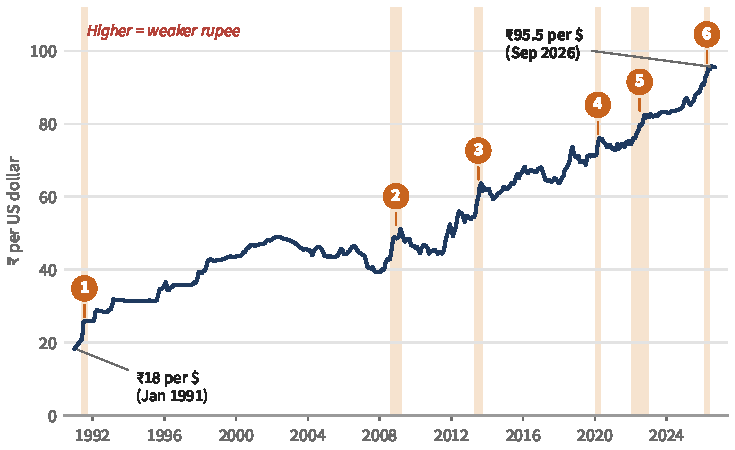
\includegraphics[width=\linewidth]{figures/rupee_history.pdf}
  \caption{The rupee against the US dollar, January 1991 to September 2026.}
  \label{fig:history}
  {\raggedright\small\sffamily Each point is the average exchange rate for one month. A rise in the line means it takes more rupees to buy one dollar, so the rupee has weakened. The shaded bands, numbered 1 to 6, mark six sharp falls in the rupee. The box `Reading the rupee's history' asks you to identify them.\par}
  \figsource{Board of Governors of the Federal Reserve System (2026a), series EXINUS, monthly averages, retrieved from FRED, 1 November 2026.}
\end{figure}

The slow part of the climb is mainly about inflation. Prices in India have usually risen faster than in the United States, which slowly makes Indian goods dearer for foreign buyers and American goods cheaper for Indians \seesec{sec:real}. Fewer dollars come in through exports, more are needed for imports, and the rupee drifts down year after year.

The sudden jumps are usually about money crossing borders. When foreigners buy Indian shares, bonds or businesses, dollars flow in; when they sell, dollars flow out. These movements are called \keyterm{capital flows}{Money that moves between countries to buy or sell financial assets, such as shares and bonds, or real assets, such as factories.}. Portfolio money is the quickest to leave \seesec{sec:forex}, which is why it matters so much for short-run swings.

What makes this money move? Very often, interest rates. Investors compare what they can earn on an American government bond with what they can earn on an Indian one. The gap between the two is the \keyterm{interest rate differential}{The difference between the interest rates paid in two countries. Funds tend to move towards the higher return, after allowing for risk.}. When the US Federal Reserve raises its interest rate, the gap narrows. Foreign investors sell Indian assets and take their dollars home, and the supply of dollars shifts to the left (Figure~\ref{fig:shocks}b). This is why a decision taken in Washington is front-page news in Mumbai.

Crude oil is the other big mover. India imports about 88 per cent of the crude oil it uses (Petroleum Planning \& Analysis Cell [PPAC], 2025). When the world price of oil rises, refiners need more dollars to buy the same number of barrels, and the demand for dollars shifts to the right (Figure~\ref{fig:shocks}a). A widening current account deficit \seesec{sec:bop} has a similar effect.

\begin{figure}[!htb]
  \centering
  \resizebox{0.92\linewidth}{!}{% Figure (Section 9, Member 4): two shocks in the market for US dollars.
% (a) oil price rise: demand shifts right, ₹85 -> ₹90.
% (b) US interest rates rise: supply shifts left, ₹85 -> ₹89.
% Same geometry as Figure 4: D: y = 3.2 - 0.8125(x - 0.4), S: y = 0.6 + 0.8125(x - 0.4).
\begin{tikzpicture}[ds, x=0.9cm]
\foreach \ox/\title in {0/{(a) World oil price rises}, 6.2/{(b) US interest rates rise}} {
  \begin{scope}[shift={(\ox,0)}]
    \draw[ds axis] (0,0) -- (0,3.7) node[above] {₹ per US dollar};
    \draw[ds axis] (0,0) -- (5,0);
    \node[below] at (2.5,0) {Quantity of US dollars};
    \node[ds title] at (-0.4,4.15) {\title};
  \end{scope}
}
% (a) demand shifts right by 1: E1 at (2.5, 2.306)
\draw[ds demand] (0.4,3.2) -- (3.6,0.6) node[below] {D\textsubscript{0}};
\draw[ds demand, ds new] (1.4,3.2) -- (4.6,0.6) node[below] {D\textsubscript{1}};
\draw[ds supply] (0.4,0.6) -- (3.6,3.2) node[above] {S};
\draw[ds shift] (2.95,1.2) -- (3.75,1.2);
\draw[ds guide] (0,1.9) -- (2,1.9) -- (2,0);
\draw[ds guide] (0,2.306) -- (2.5,2.306) -- (2.5,0);
\node[ds eq] at (2,1.9) {}; \node[below=3pt] at (2,1.9) {E\textsubscript{0}};
\node[ds eq=fxgreen] at (2.5,2.306) {}; \node[above=3pt, text=fxgreen] at (2.5,2.306) {\textbf{E\textsubscript{1}}};
\node[left] at (0,1.9) {85};
\node[left, text=fxgreen] at (0,2.306) {\textbf{90}};
% (b) supply shifts left by 0.8: E1 at (1.6, 2.225)
\begin{scope}[shift={(6.2,0)}]
  \draw[ds demand] (0.4,3.2) -- (3.6,0.6) node[below] {D};
  \draw[ds supply] (0.4,0.6) -- (3.6,3.2) node[above] {S\textsubscript{0}};
  \draw[ds supply, ds new] (0,0.925) -- (2.8,3.2) node[above] {S\textsubscript{1}};
  \draw[ds shift] (2.9,2.7) -- (2.28,2.7);
  \draw[ds guide] (0,1.9) -- (2,1.9) -- (2,0);
  \draw[ds guide] (0,2.225) -- (1.6,2.225) -- (1.6,0);
  \node[ds eq] at (2,1.9) {}; \node[right=5pt] at (2,1.9) {E\textsubscript{0}};
  \node[ds eq=fxgreen] at (1.6,2.225) {}; \node[above=3pt, text=fxgreen] at (1.6,2.225) {\textbf{E\textsubscript{1}}};
  \node[left] at (0,1.9) {85};
  \node[left, text=fxgreen] at (0,2.225) {\textbf{89}};
\end{scope}
\end{tikzpicture}
}
  \caption{Two shocks in the market for US dollars (hypothetical numbers).}
  \label{fig:shocks}
  {\raggedright\small\sffamily (a) 1. The market starts at E\textsubscript{0}, ₹85 per dollar. 2. Oil now costs more, so refiners want more dollars at every exchange rate: demand shifts right to D\textsubscript{1}. 3. At ₹85 there is excess demand for dollars, and buyers bid the price up. 4. The new equilibrium E\textsubscript{1} is at ₹90: the rupee has depreciated and more dollars change hands.\\
  (b) 1. Start again at E\textsubscript{0}, ₹85. 2. Foreign investors move funds to the United States, so fewer dollars are offered in India at every exchange rate: supply shifts left to S\textsubscript{1}. 3. The new equilibrium E\textsubscript{1} is at ₹89: the rupee has depreciated and fewer dollars change hands.\par}
  \figsource{Drawn by the authors.}
\end{figure}

Markets also look ahead. If traders expect the rupee to fall, importers rush to buy dollars today and exporters hold on to the dollars they already have. Buying or selling a currency to profit from its expected future price is called \keyterm{speculation}{Buying or selling an asset, such as a currency, in the hope of profiting from a change in its price.}. It can turn a fear into a fact: the rupee falls partly because so many people acted on the belief that it would.

Real episodes usually mix several of these forces. In the global financial crisis of 2008 and the COVID-19 panic of 2020, investors everywhere fled to the safety of the US dollar. India caused neither crisis, yet the rupee fell both times. Table~\ref{tab:moves} sums up the forces, and the box that follows asks you to read the rupee's history for yourself.

\begin{table}[!htb]
\centering\small\sffamily
\caption{What moves the rupee: a summary.}\label{tab:moves}
\begin{tabularx}{\linewidth}{@{}>{\raggedright\arraybackslash}p{38mm}>{\raggedright\arraybackslash}X>{\raggedright\arraybackslash}p{12mm}>{\raggedright\arraybackslash}p{18mm}@{}}
\toprule
\textbf{What happens} & \textbf{Effect in the market for dollars} & \textbf{₹/\$ rate} & \textbf{Rupee}\\
\midrule
Inflation in India runs ahead of US inflation & Demand rises and supply falls, slowly, over years & Rises & Depreciates\\
US interest rates rise & Supply shifts left as foreign investors take money home & Rises & Depreciates\\
Foreign investors pour money into India & Supply shifts right & Falls & Appreciates\\
World crude oil price rises & Demand shifts right & Rises & Depreciates\\
Current account deficit widens & Demand for dollars runs ahead of supply from trade & Rises & Depreciates\\
Traders expect the rupee to fall & Demand shifts right and supply shifts left & Rises & Depreciates\\
Global panic (`flight to safety') & Supply shifts left as money leaves emerging economies & Rises & Depreciates\\
\bottomrule
\end{tabularx}
\par\smallskip{\raggedright\footnotesize\sffamily\color{fxmuted}Each change is assumed to happen on its own, with everything else held constant. The opposite change has the opposite effect.\par}
\end{table}

\begin{economistsfacts}{Reading the rupee's history}
Figure~\ref{fig:history} marks six sharp jumps in the price of the dollar, numbered 1 to 6. Each matches one of the events below, which are listed in no particular order.
\begin{enumerate}[label=\Alph*., leftmargin=1.6em]
  \item The US Federal Reserve raises interest rates at its fastest pace in four decades, while war in Ukraine pushes up oil prices.
  \item India, with reserves for only about two weeks of imports, devalues the rupee.
  \item Conflict in West Asia sends crude oil above \$110 a barrel, and foreign investors sell Indian assets.
  \item A giant American investment bank collapses and a global financial crisis spreads.
  \item The US central bank hints that it will soon slow its support for the American economy, and investors pull money out of emerging markets.
  \item A new virus shuts down economies around the world.
\end{enumerate}
\textbf{1.} Match each number to an event. \textbf{2.} For each, say whether the main change was in the demand for dollars, the supply of dollars, or both. \textbf{3.} One event does not fit the demand-and-supply story. Which one, and why? (Hint: see \secref{sec:systems}.)
\answers{1--B (1991): does not fit, because the rate was cut by an official devaluation, not by the market. 2--D (2008): supply shifted left as investors fled to the dollar. 3--E (2013, the `taper tantrum'): supply shifted left as foreign money left; India's large current account deficit kept demand high. 4--F (2020): supply shifted left in a global flight to safety. 5--A (2022): both, supply left (US rate rises) and demand right (dearer oil). 6--C (2026): both, demand right (oil) and supply left (foreign investors sold Indian assets).}
\end{economistsfacts}
